\chapter{Processi e thread}
\section{Processi}
Si dice processo un istanza di un programma in esecuzione, un concetto dinamico eseguito in modo sequenziale. In un sistema multiprogrammato i processi evolvono in modo concorrente a 
causa delle risorse fisiche e logiche limitate. Il sistema operativo stesso consiste di pi\`u processi. 
\subsection{Immagine in memoria}
Il processo consiste in istruzioni (sezione Codice o Testo, la parte statica del codice), dati (sezione Dati, le variabili globali), lo Stack (chiamate a procedure e paremetri e 
variabili locali), lo Heap (la memoria allocata dinamicamente) e gli attributi (id, stato, controllo).
\subsubsection{Attributi}
All'interno del sistema operativo ogni processo \`e rappresentato dal process control block (PCB) che contiene le informazioni riguardanti lo stato del processo, il program counter, 
i valori dei registri, le informazioni sulla memoria, informazioni sullo stato dell'I/O, informazioni sull'utilizzo del sistema e informazioni di scheduling come la priori\`a. 
\subsection{Stati di un processo}
Durante la sua esecuzione un processo evolve attraverso diversi stati con un diagramma specifico al sistema operativo. Lo schema base contiene un nuovo processo che deve essere 
ammesso nel sistema, lo stato non in esecuzione che viene messo in esecuzione dall'operazione di dispatch (l'operazione inversa avviene dalla pausa). La stato finito viene ottenuto
dopo la terminazione. Un processo pu\`o essere messo in pausa a causa di un time out, caso nel quale viene messo direttamente tra i processi pronti, o essere in attesa del completamento 
di un altro processo che compie un evento per cui diventa pronto. 
\subsection{Scheduling}
Lo scheduling \`e l'operazione di selezione del processo da eseguire nella CPU al fine di garantire la multiprogrammazione (con l'obiettivo di massimizzare l'uso della CPU con pi\`u di
un processo in memoria) e il time-sharing (con l'obiettivo di commutare frequentemente la CPU tra processi in modo che ognuno creda di avere la CPU tutta per s\`e). Il long term
scheduler o job scheduler seleziona quali processi devono essere trasferiti nella coda dei processi pronti, mentre lo short-term scheduler o CPU scheduler seleziona quali sono i 
prossimi processi ad essere eseguiti e alloca la CPU di conseguenza. Il secondo \`e invocato molto di frequente e pertanto deve essere veloce, mentre il primo viene invocato meno
frequentemente e pu\`o essere lento. Il long-term scheduler controlla il grado di multiprogrammazione. 
\subsubsection{Code di scheduling}
Ogni processo \`e inserito in una serie di code: la coda dei processi pronti (ready queue) che \`e la coda dei processi pronti per l'esecuzione e la coda di un dispositivo ovvero la
coda dei processi in attesa che il dispositivo si liberi. All'inizio il processo \`e nella ready queue fino a quando non viene selezionato per essere eseguito (dispatched). Durante
l'esecuzione pu\`o accadere che:
\begin{itemize}
	\item il processo necessiti di I/O e venga inserito in una coda di un dispositivo
	\item il processo termina il quanto di tempo, viene rimosso forzatamente dalla CPU e reinserito nella ready queue
	\item il processo crea un figlio e ne attende la terminazione
	\item il processo si mette in attesa di un evento
\end{itemize}
\subsection{Operazione di dispatch}
Durante il dispatch deve avvenire un cambio di contesto: salvataggio del PCB del processo che esce e caricamento del PCB del processo che entra. Dopo questo avviene il passaggio alla
modalit\`a utente (all'inizio della fase di dispatch il sistema si trova in modalit\`a kernel). Infine avviene il salto all'istruzione da eseguire del processo appena arrivato nella
CPU.
\subsubsection{Cambio di contesto}
Il passaggio della CPU a un nuovo processo causa la registrazione dello stato del processo vecchio e il caricamento dello stato del nuovo. Il tempo necessario al cambio di contesto 
\`e un puro overhead: il sistema non compie alcun lavoro utile e la durata del cambio di contesto dipende molto dall'architettura.
\subsection{Operazioni sui processi}
\subsubsection{Creazione di un processo}
Un processo pu\`o creare un figlio che ottiene risorse dal sistema operativo o dal padre (sparizione, condivisione). Il figlio pu\`o essere eseguito in modalit\`a sincrona (il padre
attende la terminazione dei figli) o in modalit\`a asincrona (evoluzione parallela e concorrente di padre e figli). In UNIX per creare un figlio si usa:
\begin{itemize}
	\item System call \emph{fork}: crea un figlio che \`e un duplicato esatto del padre.
	\item System call \emph{exec}: carica sul figlio un programma diverso da quello del padre.
	\item System call \emph{wait}: per l'esecuzione sincrona tra pare e figlio.
\end{itemize}
\subsubsection{Terminazione di un processo}
Un processo pu\`o terminare in tre casi: quando finisce la sua esecuzione, quando \`e terminato forzatamente dal padre (per eccesso nell'uso delle risorse, perché il compito richiesto al figlio
non \`e pi\`u necessario oppure perché il padre termina e il sistema operativo non permette ai figli di sopravvivere al padre) o quando il processo \`e terminato forzatamente dal sistema operativo
(in caso di chiusura da parte dell'utente o a causa di errori). 
\subsection{Stati di un processo}
\begin{figure}[h]
	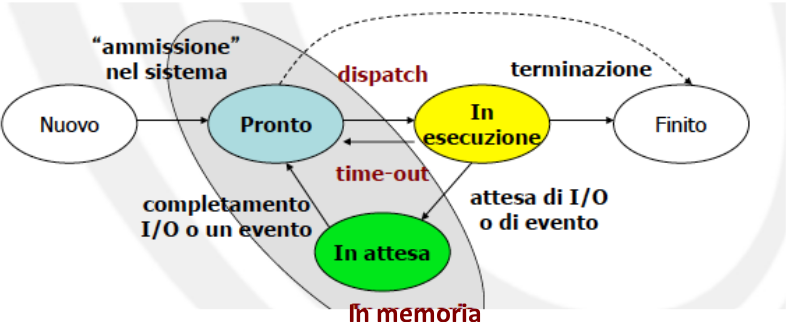
\includegraphics[width=\textwidth]{Pictures/StatiProcesso.png}
	\caption{Stack del sistema operativo}
\end{figure}
\section{Threads}
Si noti come un processo unisce i concetti del possesso delle risorse e utilizzo della CPU, caratteristiche indipendenti che possono essere considerate separatamente: si considera il 
thread come l'unit\`a minima di utilizzo della CPU e il processo come unit\`a minima di possesso delle risorse. Ad un processo sono dunque associati spazio di indirizzamento e risorse
del sistema, mentre a un singolo thread lo stato di esecuzione, contatore del programma, insieme di registri e lo stack. Le thread condividono tra di loro lo spazio di indirizzamento e
risorse e stato del processo.
\subsection{Multi-threading}
Il multithreading rappresenta la capacit\`a di un sistema operativo di supportare pi\`u thread per un singolo processo e ha come conseguenza la separazione tra flusso di esecuzione e 
spazio di indirizzamento: i processi con thread multipli hanno pi\`u flussi associati ad un singolo spazio di indirizzamento. 
\subsection{Vantaggi dei thread}
I thread permettono di ridurre il tempo di risposta in quanto il blocco di un thread permette comunque ad altri thread di continuare la propria esecuzione. Oltre a quello permettono
di condividere delle risorse in quanto thread di uno stesso processo condividono la memoria senza dover introdurre tecniche esplicite di condivisione (necessario per i processi) e 
pertanto la sincronizzazione e comunicazione risulta agevolata. La creazione, la terminazione e il contex switch risulta pi\`u veloce tra i thread rispetto che tra i processi. 
Presentano infine grandi vantaggi per quanto riguarda l'aumento di parallelismo se l'esecuzione avviene su multiprocessore. 
\subsection{Stati di un thread}
Un thread possiede gli stessi stati di un processo: pronto, in esecuzione e in attesa, ma in generale lo stato del processo pu\`o non coincidere con lo stato di un suo thread.
\subsection{Implementazione dei thread}
I thread possono essere implementati a user-level (one to many), a kernel-level (one to one) o ibrida (m to n).
\subsubsection{Thread user-level}
La gestione viene affidata alle applicazioni, il kernel ignora l'esistenza dei thread e le funzionalit\`a sono disponibili tramite una libreria di programmazione. I vantaggi di questa 
implementazione riguardano la non necessit\`a di passare in kernel-mode per utilizzare i thread prevenendo due mode switch aumentando l'efficienza, la possibilità di variare il meccanismo di scheduling in base alle necessit\`a applicative e quella di essere eseguiti su qualsiasi sistema operativo senza modificare il kernel. Come svantaggi presentano il fatto che il blocco di 
un thread blocca l'intero processo (superabile con accorgimenti specifici) e che non \`e possibile sfruttare il multiprocessore: lo scheduling di un thread \`e presente sempre sullo stesso
processore: un solo thread \`e in esecuzione per ogni processo.
\subsubsection{Thread kernel-level}
La gestione viene affidata al kernel e le applicazioni usano i thread tramite system call. I vantaggi sono lo scheduling a livello thread in quanto il blocco di un thread non blocca
l'intero processo, pi\`u thread dello stesso processo possono essere in esecuzione in contemporanea su CPU diverse e le funzioni del sistema operativo stesse possono essere  
multithreaded. Come svantaggi presenta la scarsa efficienza in quanto il passaggio tra i thread implica un passaggio attraverso il kernel.
\subsection{La libreria posix pthreads}
Per usare i pthreads in un programma C \`e necessario includere la libreria \emph{$<$pthread.h$>$} e occorre linkare la libreria libpthread usando l'opzione \emph{-pthread}. 
\subsubsection{Creazione di un thread}
Un thread ha vari attributi che possono essere cambiati come la sua priorit\`a e la dimensione del suo stack contenuti in un oggetto di tipo \emph{pthread\_attr\_t} e la system call
\emph{int pthread\_attr\_init(pthread\_attr\_t *attr);} inizializza con i valori di default un contenitore di attributi \emph{*attr} che pu\`o essere passato alla system call per creare
un nuovo thread. La creazione vera e propria avviene tramite la system call \emph{pthread\_create} che accetta quattro argomenti:
\begin{itemize}
	\item Una variabile di tipo \emph{pthread\_t} che contiene l'identificativo del thread che viene creato.
	\item Un oggetto \emph{*attr} che contiene gli attributi da dare al thread creato (\emph{NULL} per i default).
	\item Un puntatore alla routine che contiene il codice che deve essere eseguito dal thread.
	\item Un puntatore all'argomento che si vuole passare alla routine stessa.
\end{itemize}
\subsubsection{Terminazione di un thread}
Un thread termina quando finisce il codice della routine specificata all'atto della creazione del thread stesso o quando nel codice della routine si chiama la system call di terminazione
\emph{void pthread\_exit(void *value\_ptr);}. Quando termina il thread restituisce il valore di return specificato nella routine o se chiama la system call il valore passato a quella
come argomento. 
\subsubsection{Sincronizzazione fra thread}
Un thread pu\`o sospendersi in attesa della terminazione di un altro thread chiamando la system call \emph{int pthread\_join(pthread\_t thread, void **value\_ptr);} dove il primo 
argomento \`e l'identificativo del thread di cui si vuole attendere la terminazione (appartenente allo stesso processo) e il secondo valore restituito dal thread che termina. 
\subsubsection{Sincronizzazione fra thread}
\paragraph{Condivisione dello spazio logico}
Due thread dello stesso processo condividono lo stesso spazio di indirizzamento e le stesse variabili, cosa che nei processi tradizionali \`e possibile solo usando esplicitamente un
segmento di memoria condivisa. 
\paragraph{Sincronizzazione dell'esecuzione}
La sincronizzazione pu\`o avvenire attraverso diversi strumenti come i semafori (non disponibili nell'ultima versione dello standard) e meccanismi di sincronizzazione strutturati come
le variabili condizionali. 
\section{Relazione tra processi}
Nei processi indipendenti si nota un'esecuzione deterministica che dipende solo dal proprio input che non influenza, n\`e viene influenzata da altri processi con i quali non avviene
nessuna condivisione dei dati. Nei processi cooperanti invece un processo pu\`o essere influenzato e influenzare altri processi e l'esecuzione risulta non deterministica e non 
riproducibile. I processi cooperanti sono naturalmente necessari per la condivisione di informazioni, permettono di accelerare il calcolo eseguendo parallelamente subtask su 
multiprocessore, permettono la modularit\`a con funzioni distinte su vari processi e sono convenienti. Si devono naturalmente stabilire dei modelli di comunicazione rigorosi: lo scambio
di messaggi e la condivisione della memoria.
\subsection{Scambio di messaggi}
Il passaggio di messaggi \`e un meccanismo utilizzato dai processi per comunicare e sincronizzare le loro azioni e in questo caso i processi comunicano tra loro senza condividere 
variabili. Le IPC forniscono le operazioni di \emph{send(message)} e di \emph{receive(message)} con la lunghezza del messaggio fissa o variabile. Se $P$ e $Q$ desiderano comunicare 
devono stabilire un canale di comunicazione e scambiarsi messaggi attraverso send/receive. Il canale di comunicazione deve essere implementato naturalmente sia in maniera fisica che
logica. 
\subsubsection{Comunicazioni dirette}
Nella comunicazione i processi devono nominarsi esplicitamente e pu\`o essere simmetrica: \emph{send(P1, message)} e \emph{receive(P2, message)} dove P1 e P2 sono gli id rispettivamente
di destinatario e mittente o pu\`o essere asimmetrica: \emph{send(P1, message)} e \emph{receive(id, message)} dove in id viene salvato il nome del processo che ha eseguito la send. Si
nota come se un processo cambia nome si devono ricodificare tutti i messaggi di send e receive.
\subsubsection{Comunicazioni indirette}
I messaggi sono spediti e ricevuti da mailboxes o porte tali che ogni mailbox ha un unico id e i processi possono comunicare solo se condividono una mailbox. Le operazioni permettono
di creare una nuova mailbox, \emph{send} e \emph{receive} tramite mailbox ed eliminare una mailbox. Le primitive sono definite come \emph{send(A, message)}: spedire un messaggio alla
mailbox A e \emph{receive(A, message)}, ricevere un messaggio dalla mailbox A. Il canale di comunicazione pu\`o essere stabilito solo se i processi condividono una mailbox comune, 
ogni canale pu\`o essere associato a molti processi, ogni coppia di processi pu\`o condividere molti canali di comunicazione e i canali possono essere unidirezionali o bi-direzionali. Le
concorrenze rispetto alla ricezione si risolvono permettendo ad un canale di essere associato al pi\`u con due processi, permettendo a un solo processo alla volta di eseguire la 
ricezione o permettendo al sistema di selezionare in modo arbitrario il ricevente: il mittente \`e notificato di chi ha ricevuto il messaggio. 
\subsubsection{Sincronizzazione}
Lo scambio di messaggi pu\`o essere bloccante o non bloccante.
\paragraph{Bloccante (sincrono)}
La send bloccante blocca il mittente fino a che il messaggio \`e ricevuto e la receive bloccante blocca il ricevente fino a che il messaggio \`e disponibile. 
\paragraph{Non bloccante (asincrono)}
La send non bloccante permette al mittente di spedire il messaggio e continuare la sua esecuzione e la receive non bloccante permette al ricevente di ricevere un messaggio valido o 
nulla permettendogli di continuare la sua esecuzione in ogni caso. 
\subsection{Memoria condivisa}
In POSIX il processo crea prima il segmento di memoria condivisa \emph{segment id = shmget(IPC\_PRIVATE, size, S\_IRUSR $|$ S\_IWUSR);} il processo che vuole accedere alla memoria
condivisa deve attaccarsi: \emph{shared memory = (char *) shmat(id, NULL, 0);} ora il processo pu\`o scrivere nel segmento condiviso attraverso \emph{sprintf} e quando ha finito il 
processo stacca il segmento di memoria dal proprio spazio di indirizzi: \emph{shmdt(shared memory);} e per rimuovere il segmento di memoria si usa 
\emph{shmctl(shm\_id, IPC\_RMID, NULL);}
\subsubsection{Pipe}
Le pipe agiscono come condotte che permettono a due processi di comunicare.
\paragraph{Pipe ordinarie}
Le pipe ordinarie permettono la comunicazione in stile produttore-consumatore: il produttore scrive ad un'estremit\`a, mentre il consumatore legge all'altra estremit\`a. Sono 
unidirezionali e richiedono una relazione parent-child tra i processi comunicanti. 
\paragraph{Pipe con nome}
Le pipe con nome permettono comunicazioni bidirezionali senza relazione parent-child. Sono utilizzabili da pi\`u processi. 
\section{Gestione dei processi del sistema operativo}
Il sistema operativo \`e un programma e il kernel pu\`o essere eseguito separatamente, all'interno di un processo utente o come processo. 
\subsection{Kernel separato}
Il kernel viene eseguito al di fuori di ogni processo con uno spazio riservato in memoria, prende il controllo del sistema ed \`e sempre in esecuzione in modo privilegiato. Il concetto
di processo viene applicato solo ai processi utente.
\subsection{Kernel in processi utente}
Si considerano i servizi del sistema operativo come procedure chiamabili da programmi utente accessibili in modalit\`a protetta (kernel mode). L'immagine dei processi prevede il 
kernel stack per gestire il funzionamento di un processo in modalit\`a protetta e il codice e dati del sistema operativo condiviso tra i processi. Offre un vantaggio di efficienza in
quanto dopo interrupt o trap durante l'esecuzione \`e necessario un solo mode switch in cui il sistema passa da user mode a kernel mode e viene eseguita la parte di codice relativa al
sistema operativo senza context switch. Dopo il completamento del suo lavoro il sistema operativo pu\`o decidere di riattivare lo stesso processo utente (mode switch) o un altro 
(context switch). 
\subsection{Kernel come processo}
Si considerano i servizi del sistema operativo come processi individuali eseguiti in modalit\`a protetta, una minima parte del sistema operativo deve essere eseguita al di fuori di
tutti i processi (lo scheduler). \`E vantaggioso per sistemi multiprocessore dove processi del sistema operativo possono essere eseguiti su un processore ad hoc. 
